\documentclass[12pt]{article} %[a4paper]{article}

\usepackage{caption}
\usepackage{subcaption}
% accetta caratteri complicati tipo vocali accentate
\usepackage[T1]{fontenc}
\usepackage[utf8]{inputenc}


%collegamenti ipertestuali
\usepackage{hyperref}

%tabelle
\usepackage{booktabs}
\usepackage{caption}

%grafici
\usepackage{graphicx}
\usepackage{subcaption}

%matematica
\usepackage{mathtools}
\usepackage{amsmath}

%stile di pagine
\pagestyle{plain} %headings?

%Notes
\usepackage{fancyhdr}
\usepackage{wrapfig}% layout
\usepackage{graphicx}				%import images
\usepackage[export]{adjustbox}
\graphicspath{{Images/}}									% permet d'aller chercher des fichiers (utilise graphicx)
\usepackage[colorinlistoftodos]{todonotes}						% pour faire des notes	
\usepackage[toc,page]{appendix}
\usepackage{caption}
\usepackage{subcaption}


\usepackage{enumerate}
\usepackage[english]{babel}
\usepackage[utf8]{inputenc}
\usepackage[T1]{fontenc}
\usepackage{lmodern}
\usepackage{amsmath,amsfonts,amssymb}
\usepackage{graphicx}
\usepackage{geometry}
\geometry{a4paper}
\usepackage[parfill]{parskip}
\usepackage{graphicx}
\usepackage{amssymb}
\usepackage{epstopdf}
\usepackage{color}
\usepackage[tt]{titlepic}
\usepackage{fancyhdr}
\usepackage{enumerate}
\usepackage{lastpage}
\usepackage[labelformat=simple]{subcaption}
%\usepackage{subfigure}
\usepackage{caption}
\usepackage{bm}
\usepackage{verbatim}
\usepackage{listings}
\usepackage{tasks}
\usepackage{float}
%\pagenumbering{gobble}
\numberwithin{equation}{subsection}

\begin{document}

\newcommand*\xbar[1]{%
  \hbox{%
    \vbox{%
      \hrule height 0.5pt % The actual bar
      \kern0.5ex%         % Distance between bar and symbol
      \hbox{%
        \kern-0.1em%      % Shortening on the left side
        \ensuremath{#1}%
        \kern-0.5em%      % Shortening on the right side
      }%
    }%
  }%
} 

%\interfootnotelinepenalty=10000
\begin{titlepage}
	\vspace{20mm}
	\begin{center}
		
\includegraphics[width=5cm]{Figures/EPFL_LOG.pdf}\\
		\vspace{2cm}
		%{\large{\bf }}\\
		\vspace{5mm}
		{\LARGE{\bf A Portfolio Allocation Framework \\ \vspace{5pt} for Algorithmic Trading Strategies}}\\
		\vspace{3mm}
		{\large{\bf Master Project}}\\
		\vspace{19mm} {\large{\bf In cooperation with NAFORA SA}}
	\end{center}
	\vspace{20mm}
	\par
	\noindent
	%\begin{center}

			{\large{\bf Realized by: \\
					ALESSANDRO DANIELE FORLONI\\ \vspace{10pt}
					
					\bf Supervised by: \\
					YILIN HU and SEMYON MALAMUD\\ \vspace{10pt}
				}}
	%\end{center}
	
	\vspace{5mm}
	\begin{center}
		{\large{\bf Academic Year\\
				2017/2018 }}
	\end{center}
\end{titlepage}

\newpage
\tableofcontents

\newpage

\section*{Acnkowledgments}
%\addcontentsline{toc}{section}{Acnowledgments}

\section{Introduction}\label{intro}
%\addcontentsline{toc}{section}{Introduction}

In this thesis we address the challenge of portfolio allocation applied to a set of trading algorithms. The aim here is to allocate risk to many algorithmic trading strategies on a weekly basis. The problem is to be solved in two seprate parts: firstly address at any moment in time which strategies out of the many available to put into production and at last assign proper risk weights to these strategies. We will see that both the steps are to be addressed with care as none of these problem if solved alone can achieve satisfactory results. All the results will be compared with a proper benchmark that mimics the current non-systematic allocation strategy. If the procedure is will be implemented it will make the whole investing process completely systematic. The weekly allocation period is chosen as it fits at best the charachteristics of the market of interest and it avoids incurring in excessive transaction costs arousing from daily rebalancing of the portfolio that would erase any improvement given by the selection methodology.\\
The challenges that have been faced include the abundance of strategies and the well known issue that alpha in algorithmic trading strategies is not everlasting. There is a point in time at which any strategy will stop working and will necessarily be switched off, on the other hand, as a reaction to market changes, some strategies that in the past performed poorly might become alpha generators. Achieving optimal timing in putting into production and swithcing off the strategies represents a challenge but also an opportunity to substantially increase trading performance.This task is hard to perform in other ways than algorithmic selection because often what is selected might not look intuitive to trade at first sight. Inter-market relationships change through time. \todo{CONTROLLA CHE NON SIA UNA CAZZATA} For example, if one is trading on the well known relationship between Gold and US Government Bond (which is expected to be stedily meaningful and potentially a good source of alpha), it might be that due to some specific event this correlation breaks down, changing all the underlying market-dynamics and making the algorithms unprofitable. Moreover, in some cases, a certain strategy might perform really well for years until somebody in the market strats exploiting it systematically and at high frequency bringing liquidity and margin for trading out of the scope of hedge funds. In such cases detecting a switching point in the performance of strategies is of crucial importance.\\


%IF WE NEED TO CITE SOMETHING USE: \cite{example}.





\subsection{Literature Review}
%\addcontentsline{toc}{subsection}{Literature Review}

The problem of portfolio optimization is one of the oldest and most discussed topics in finance. The traditional theory that has been just discussed has been developed at first by Harry Markowitz who won the Nobel Prize for his article \textit{Portfolio Selection} in 1952 \cite{Markowitz}. The Modern Portfolio Theory that was developed in those years is actually a milestone of finance, and still today it is regarded as the baseline for portfolio managers. Unfortunately, Markowitz allocation procedures have some drawbacks, mainly relative to the numerical instability of the estimation of asset returns. Some scholars improved through the years the models trying to add stability. In 1992 a huge step forward was made by Fisher Black and Robert Litterman with their article \textit{Global Portfolio Optimization} \cite{black_litterman} that merged the CAPM equilibrium theory with the mean-variance optimization proposed by Markowitz. Their idea was that incorporating meaningful information coming from CAPM and personal views of portfolio managers would solve the issues of unreasonableness of quantitative portfolios. More recently, an additional step was made by Olivier Ledoit and Michael Wolf whose contribution was to improve the global performance of covariance matrices by introducing the idea of \textit{shrinkage}. This method allows to have more stable covariance matrices and therefore making the Markowitz framework more stable and applicable.  \\
Many experts from different fields have worked to enrich the knowledge in this specific area. A well-known example is that of Professor Cover, whose work is recognized as one of the finest attempts tu use signal theory in portfolio allocation. With his article \textit{Universal Portfolios} \cite{universal_portfolios} he builds a portfolio, that in terms of performance, asympthotically beats the best stock over a given set of stocks. The interesting part of cover's work is that he attempts to solve the portfolio optimization puzzle in a non-parametric way, using robust results, this unfortunately comes at the expense of not universal applicability.\\
Recently, with the advent of Machine Learning, many experts started applying powerful algorithms to portfolio selection with interesting results. Any kind of use has been made, from forecasting returns to allocate risk to cluster assets to create well-diversified portfolios. The increase of computational power has allowed to test on large scale portfolios complex algorithms like genetic learning models or neural networks. These have been used in many ways, for example some researchers in the US have trained a one-layer recurrent neural network to dynamically optimize a portfolio \cite{NN_1}. Others tried to forecast asset returns with a specific Hopfield Neural network to input into a traditional mean-variance Markowitz style optimization \cite{NN_2}.\\
Despite their out-of-sample results are not outstanding, these pieces of work set with others a new path for portfolio optimization that extracts the most information out of the available data. We will follow this path trying to optimize our portfolio using the most information as possible. In particular we will follow the approach of some researches in te area of genetic algorithms \cite{genetic_1} and that of Marcos Lopez de Prado, that aims at building well-diversified portfolios with unsupervised clustering methods \cite{HRP}.\\
More than 50 years after the first attempt to address the issue of portfolio selection, Markowitz models are still regarded as the baseline model around which all the theory is built. These models still have relevant real-world issues such as ignorance of transaction costs and high instability of the portfolio, but are really intuitive and representative of the dynamics of a rational investor.  


\subsection{Our Approach}
%\addcontentsline{toc}{subsection}{Our Approach}

The "schedule" we set at the beginning is to find firstly a satisfactory method to switch strategies on and off and then move to the part of weight allocation. We will consider the first step to be completed once the resulting selection allows for efficient trading of around a hundredth of strategies with at least half of the trading days with positive pnl.\\
\todo{QUI E' TUTTO DA VERIFICARE ED AGGIORNARE}
To achieve this step a simple and robust feature-based approach has been used. We decided not to try to use any hard-core machine learning type approach to reduce the risk of overfitting and to fit the specificity of the problem. In fact, the abundance of strategies and the lack of a long samples would have made traning a machine learning method cumbersome and time-consuming.\\
Before getting into this part, relevant features are needed to give some predictive insight to our models. To this end we built several different features and evaluated their predictive power through a \textit{Random Forest Tree} (details of this model will be provided later).\\
For what concerns assigning the weights we developed two different approaches, one of which is more computationally oriented and the other is more diversification-driven. The first approach is to train a genetic portfolio allocator that will select the best portfolio in-sample and then apply iy out of sample. The second approach is based on clustering, and aims at reducing as much as possible the realized variance of the portfolio.\\

Aggiungi altri dettagli: cioè quello che aggiungiamo rispetto alla teoria classica:
\begin{itemize}
	\item cross-validation
	\item robust feature importance
	\item rigorous separation of in-sample, out of sample and production set
	\item unsupervised methods with little assumptions
\end{itemize}


\subsection{The data}
%\addcontentsline{toc}{subsection}{The Data}

As mentioned before the dataset at hand consists of 13000 simulated strategies, based on mean-reversion. All these strategies are trading one futures against another one looking for relative mispricings. This number of strategies comes out of a simulation of all possible trading pairs among roughly 150 futures traded worldwide. The huge diversity among these strategies makes it hard to find a unique model to allocate risk among all of them. Diversification has to be applied not only to asset classes, but also taking into account type of algorithms, trading latency and underlying country or region of exposure.\\
The data spans through almost six years, from January 2012 to August 2017. To perform the studies, the final year has been dropped to be used as a final validation set (also referred to as production set). The first remaining chunk has been divided into train and test set.\\
We also decided to remove any strategy involved in swiss franc trading, to avoid our results to be biased by the famous drop that happened on the 15th of January 2015. We don't want to penalize or advantage any strategy that happened to be trading the swiss franc in either long or short side in that day because we believe that was a statistically unpredictable event. There is no guarantee that such an event could be forecasted only with information coming from strategy performance.\\

\subsection{Some Descriptive Statistics}
%\addcontentsline{toc}{subsubsection}{Some Descriptive Statistics}

Here we want to give a taste of what our data looks like. We first run a code that computes sample statistics for all the strategies. The results are exposed in Table 1. 

\begin{table}
	\centering
	\begin{tabular}{c|c|c|c|c|c}
		Statistic   & Mean & Median & Min & Max & IQR \\\hline
		Mean Return & -0.0002 & -0.0002 & -0.0032 & 0.0024 & 0.0002 \\ 
		Skew        & -1.9393 & -1.698 & -34.2374 & 21.119 & 2.5754 \\ 
		Kurtosis    & 56.9226 & 25.5496 & -5.4507 & 1202.95 & 37.851 \\ 
		Sharpe Ratio& -1.3653 & -1.1725 & -20.0072 & 15.547 & 1.4080 \\ 
		Sortino     &-1.3514 & -1.1808 & -32.9069 & 40.322 & 1.3692 \\ 
	\end{tabular}
	\caption{\label{tab:widgets} Global strategy statistics.}
\end{table}

We can see how on average the mean return per strategy is negative. The sharpe ratio of course follows this pattern as well. On the other hand we notice how some sharpes are very high (e have peaks at around 15 on the wole history!). Here an important remark must be made, many strategies with good performance seem really appealing, but for several reasons might not be tradable due to liquidity issues, regulation or asynchronization of quotes data.\\
Back to our statistical analysis, we notice how the skew and kurtosis reach extreme values, signaling that the returns of these strategies might not be normally distributed. To this end we conducted a Shapiro-Wilks normality test for each strategy, where the null Hypothesis of normality is challenged (for details on this procedure refer to the Appendix). The results are the following:

We can observe that for the majority of the cases the normality hypothesis is rejected. Some strategies survive the test, but a deeper analysis supports the idea that this is caused by a lack of data for these strategies. 

\todo{AGGIUNGI STYLIZED FACTS PER CONFRONTARE CON RITORNI SOLITI}
\todo{AGGIUNGIGRAFICO AUTOCORRELATION STRATEGIE}

\subsection{Data Cleaning}

Before moving to implement any kind of model we need to make sure the data is clean and usable.\\
We first noticed that many strategies traded very rarely filling the data only with NaNs (Not a number), we removed these strategies from the data. A lot of daily PnLs were filled with zeros, in 90\% of the cases this happens on sundays and Saturdays. In such cases not all the strategies are not trading, so what we did was to bring the weekend PnL back to Friday and accumulate it there. This is possible since strategies are trading at weekends for very little amounts of time. At this point we could drop the entire weekends, the remaining 10\% of missing data was due to holidays or data actually missing, so we kept NaNs instead of the zeros values to keep the distribution on the trading days unchanged.\\  
Secondarily, the data comprises many different strategies backtested with different levels of risk, to ba able to compare them we need to scale their PnLs by their standard deviations.\\
At last we took the decision to drop some strategies, like the ones trading the Swiss franc, as it is known on the 2nd of February 2015 the Swiss frank soared in few minutes against any currency as soon as the Swiss National Bank removed the peg it had against the developed currencies. This resulted in a huge drawdowns or gains for many strategies depending on the position they had in the Swiss currency at the moment of the removal of the peg. We decide to remove these strategies as the event was completely unpredictable and no sharpe ratio or feature-based rule could make a strategy stop from trading in that case. We don't want to bias our results towards strategies that accidentally were long the Swiss franc on that moment, but we also don't want to penalize a strategy just because it was trading on a short position the Swiss Currency. At the cost of reducing out dataset (removing roughly 20 strategies) we have a more usable and reliable dataset.

\section{Classic Portfolio Theory}

\subsection{Risk and Return}

We want to establish the classical Portfolio Theory as a starting point of our work. Understanding the advantages and drawbacks of this theory will allow us to better explain some choices that have been made while developing our portfolio model. As for any rational investor we try to think in terms of risk and return. The return is a measure of how much money we will make investing in our portfolio, while the risk is a measure of how unstable our money-making model is. The latter is traditionally measured in terms of variance of portfolio returns, that's why we refer to a \textit{Mean-Variance} problem. We will illustrate later how covariance between assets in a portfolio plays a crucial role. The idea is that given a certain level of risk we will try to get out the highest return, or on the other direction, given a certain level of desired return, we will try to minimize the risk of our portfolio. The traditional Markowitz theory establishes a clear and intuitive relationship between risk and return that allows any investor to find an optimal allocation given a certain level of risk or return.\\
For our specific case, where strategies are our assets to which we allocate risk we will consider as return the amount of PnL given by a strategy on a certain day, divided by the amount of capital allocated to the strategy.
$$
r_t = \frac{PnL_i}{Allocated \quad capital}
$$
So our expected return will be:
$$
\mu = \frac{1}{N}\sum\limits_{i=1}^N r_i
$$
On the other hand, a simple measure of risk will be the standard deviation of returns:
$$
\sigma = \frac{1}{N}\sum\limits_{i=1}^N (r_i - \mu)^2
$$

We will here make a fundamental assumption, since it is arguably extremely hard to forecast future returns of strategies, we will consider past returns as a proxy for future returns.\\

\subsection{A simple two-asset example}

Let's adapt to our context a simple portfolio optimization problem. Let's consider two assets, in our case two algorithmic mean-reversion strategies (A and B for simplicity). For the moment, we consider a simple example where both the strategies have the same expected return $\mu_A = \mu_B = \mu$.
The two strategies have a certain level of risk (measured historically): $\sigma_A$ and $\sigma_B$. Moreover (and more importantly) the two strategies exhibit in their PnL history a certain correlation expressed by the pearson coefficient $\rho$.\\
Our portfolio will be a combination of A and B in a way that we allocate capital to both the strategies. The weight will be given in percentage terms ($\omega_A$ and $\omega_B$), that means, that we don't specify how much money will be put in the market, but we care about how will be the composition of the portfolio given a certain amount of capital.
$$
\Pi = \omega_A r_A + \omega_B r_B
$$

Here it is important to state clearly that we evaluate the portfolio in terms of risk-return trade-off and not only absolute return, therefore this modelling of a portfolio fits the problem.\\
We will work now with variances instead of standard deviations because it comes more natural for calculations, and being the standard deviation a monotonic transformation of variance, the results will still apply. For us $r_A$ and $r_B$ are two potentially correlated random variables.\\
The return on out portfolio will be:

\begin{equation} \label{portfolio_return}
\mu_\Pi = \omega_A \mu_A + \omega_B \mu_B 
\end{equation} 

While the variance of our portfolio will be as follows:

\begin{equation} \label{portfolio_var}
\sigma^2_\Pi = \omega_A^2 \sigma_A^2 + \omega_B^2 \sigma_B^2 + 2\rho \omega_A \omega_B\sigma_A \sigma_B
\end{equation} 

Here we can see how the correlation coefficient can actually help reduce the variance of the portfolio. To dig more in depth let's consider impose the natural constraint that $\omega_A$ and $\omega_B$ constitute the entire portfolio:


\begin{equation} \label{eq1}
\begin{split}
\sigma^2_\Pi &= \omega_A^2 \sigma_A^2 + (1 - \omega_A)^2 \sigma_B^2 + 2\rho \omega_A (1 - \omega_A)\sigma_A \sigma_B \\
             & = \omega_A^2(\sigma_A^2 - 2\rho \sigma_A \sigma_B + \sigma_B^2) + 2\omega_A(\rho \sigma_A \sigma_B - \sigma_B^2) + \sigma_B^2
\end{split}
\end{equation}

We will now solve for the optimal portfolio minimizing the variance: 

\begin{equation} \label{eq2}
\frac{\partial \sigma^2_\Pi }{\partial \omega_A} = 2\omega_A(\sigma_A^2 - 2\rho \sigma_A \sigma_B + \sigma_B^2) + 2(\rho \sigma_A \sigma_B - \sigma_B^2) = 0
\end{equation}

This yields:

\begin{equation} \label{eq3}
\omega_A = \frac{\sigma_B^2-\rho \sigma_A \sigma_B}{\sigma_A^2 - 2\rho \sigma_A \sigma_B + \sigma_B^2}
\end{equation}

We can check that this is actually a global minima by evaluating the second derivative:

\begin{equation} \label{eq_second_derivative}
\displaystyle \frac{\partial^2 \sigma^2_\Pi }{\partial \omega_A^2} = 2(\sigma_A^2 - 2\rho \sigma_A \sigma_B + \sigma_B^2) >= 0 \qquad \forall \lvert \rho \rvert <= 1
\end{equation}

We will analyze these results with different values of $\rho$ to give some economic intuition. Let's start from the basic case:
$\rho = 0$ that means the two strategies are uncorrelated. In this case \eqref{eq3} becomes:

\begin{equation} \label{eq_rho_zero}
\omega_A = \frac{\sigma_B^2}{\sigma_A^2 + \sigma_B^2}
\end{equation}

That means that weights are directly proportional two the variance of the other asset, or in other words, the higher the variance of an asset, the lower it's weight in the portfolio. In this case the overall variance of the portfolio will be simply a weighted average of the variances of the assets.\\

Let's now consider the case where the two assets are perfectly correlated ($\rho = 1$).\\
In this case \eqref{eq3} becomes:

\begin{equation}
\omega_A = \frac{\sigma_B^2-\sigma_A \sigma_B}{\sigma_A^2 - 2\sigma_A \sigma_B + \sigma_B^2} = \frac{\sigma_B}{\sigma_B - \sigma_A}
\end{equation}
 
Which is an interesting case if $\sigma_A=\sigma_B$ as the solution is non defined, and from equation \eqref{eq_second_derivative} we can see that the optimization line is flat, therefore any combination of portfolios will be "optimal".\\
At last, let's consider the most interesting case: when $\rho = -1$. In this case \eqref{eq3} becomes:

\begin{equation}
\omega_A = \frac{\sigma_B^2-\sigma_A \sigma_B}{\sigma_A^2 + 2\sigma_A \sigma_B + \sigma_B^2} = \frac{\sigma_B}{\sigma_B + \sigma_A}
\end{equation}

Where the optimal weight on one strategy is directly proportional to the standard deviation of the other strategy. It is interesting to observe the total variance of the portfolio, using \eqref{portfolio_var}:

\begin{equation} 
\sigma^2_\Pi = \left(\frac{\sigma_B}{\sigma_B + \sigma_A}\right)^2 \sigma_A^2 +  \left(\frac{\sigma_A}{\sigma_B + \sigma_A}\right)^2        \sigma_B^2 - 2 \left(\frac{\sigma_B}{\sigma_B + \sigma_A}\right)  \left(\frac{\sigma_A}{\sigma_B + \sigma_A}\right)\sigma_A \sigma_B = 0
\end{equation}

In this extreme case we can find a portfolio with zero variance!
Anyway, the key take away is that with correlations smaller than one we can achieve portfolio variances that are lower than just a simple weighted average of the variances. This is referred to as the \textit{Diversification Benefit}. We spread out the risk in different points in time resulting in a portfolio that is well-diversified and compensates losses on some assets with gains on other strategies.\\
For our prject another point of view is that given a certain correlation we can almost always find a portfolio that minimizes the variance for a given level of return.\\

\subsection{Extending to N assets}

We extend our calculations to the case of N assets. The ultimate goal is to find a combination of weights that minimizes the variance for each level of return we set. We will arrive to show that this can be achieved, and all the portfolio will lie on a parabola in a mean return-variance plane.\\
First we set some notation: let $\mathbf{\Sigma}$ be the covariance matrix of out strategies, it will be a matrix of the form:

$$
\mathbf{\Sigma}_{i,j} = 
\begin{pmatrix}
\sigma_{1}^2 & \rho_{1,2}\sigma_1\sigma_2 & \cdots & \rho_{1,n}\sigma_1\sigma_n \\
\rho_{1,2}\sigma_2\sigma_1 & \sigma_2^2 &   \cdots & \rho_{2,n}\sigma_2\sigma_n \\
\vdots  & \vdots  & \ddots & \vdots  \\
\rho_{n,1}\sigma_n\sigma_1 & \rho_{n,2}\sigma_n\sigma_2 & \cdots & \sigma_n^2 
\end{pmatrix}
$$

While $\mathbf{u}$ will be the vectors of expected returns of each strategy:

$$
\mathbf{u}_{i} = 
\begin{pmatrix}
\mu_1 & \mu_2 & \cdots & \mu_n  
\end{pmatrix}
$$

We will allocate capital expressed in percentage terms expressed by the vector 
$\mathbf{w} = \begin{bmatrix} w_1 & w_2 & \cdots & w_n \end{bmatrix}$ such that $\mathbf{w}^\top \mathbf{1} = 1$.\\
Now it is just about solving a linear optimization problem:

\begin{equation} \label{min_problem}
min \quad \frac{1}{2}\mathbf{w}^\top\mathbf{\Sigma}\mathbf{w} \qquad s.t. \qquad \mathbf{w}^\top \mathbf{1} = 1 \quad \mathbf{w}^\top \mathbf{u} = \bar{\mu}
\end{equation}

Let's write the lagrangean:

\begin{equation} \label{lagrangean}
\mathcal{L} =  \frac{1}{2}\mathbf{w}^\top\mathbf{\Sigma}\mathbf{w} -\xi(\mathbf{w}^\top \mathbf{1} - 1) - \lambda(\mathbf{w}^\top \mathbf{u} - \bar{\mu})
\end{equation}

We can immediately get the F.O.C.s:

\begin{equation} \label{focs}
\begin{split}
\frac{\partial \mathcal{L}}{\partial \mathbf{w}} &= \mathbf{\Sigma}\mathbf{w}  - \xi\mathbf{1} - \lambda\mathbf{u} = 0\\
\frac{\partial \mathcal{L}}{\partial \xi} &= \mathbf{w}^\top \mathbf{1} - 1 = 0\\
\frac{\partial \mathcal{L}}{\partial \lambda} &= \mathbf{w}^\top \mathbf{u} - \bar{\mu} = 0
\end{split}
\end{equation}

From the first F.O.C. we get:

\begin{equation} \label{first_result}
\mathbf{w} = \xi\mathbf{\Sigma}^{-1}\mathbf{1} + \lambda\mathbf{\Sigma}^{-1}\mathbf{u}
\end{equation}

Substituting \eqref{first_result} into the other two F.O.C.s we get the following system of equations:

\begin{equation} \label{focs}
\begin{split}
\xi \mathbf{1}^\top \mathbf{\Sigma}^{-1}\mathbf{1} + \lambda \mathbf{u}^\top \mathbf{\Sigma}^{-1}\mathbf{1} &= 1\\
\xi \mathbf{1}^\top \mathbf{\Sigma}^{-1}\mathbf{u} + \lambda \mathbf{u}^\top \mathbf{\Sigma}^{-1}\mathbf{u} &= \bar{\mu}
\end{split}
\end{equation}

Let's introduce the following notation:
$$
A = \mathbf{u}^\top \mathbf{\Sigma}^{-1}\mathbf{u} \qquad A = \mathbf{u}^\top \mathbf{\Sigma}^{-1}\mathbf{1} \qquad C = \mathbf{1}^\top \mathbf{\Sigma}^{-1}\mathbf{1} \qquad D = AC - B^2
$$

We rewrite the two equations:

\begin{equation} \label{focs_rewritten}
\begin{split}
\xi C + \lambda B &= 1\\
\xi B + \lambda A &= \bar{\mu}
\end{split}
\end{equation}

From which we can easily find that

\begin{equation} 
	\begin{split}
\lambda &= \frac{C\bar{\mu} - B}{D}\\
\xi     &= \frac{A - \bar{\mu}B}{D}
\end{split}
\end{equation}

We can plug this result into \eqref{first_result} to obtain a complete formula for $\mathbf{w}$:

\begin{equation} \label{final_result}
\mathbf{w} = \frac{A - \bar{\mu}B}{D}\mathbf{\Sigma}^{-1}\mathbf{1} + \frac{C\bar{\mu} - B}{D}\mathbf{\Sigma}^{-1}\mathbf{u}
\end{equation}

One can prove that the resulting variance of the portfolio is of the form:

\begin{equation} \label{N_portfolio_variance}
\sigma^2_{\Pi} = \mathbf{w}^\top \mathbf{\Sigma}\mathbf{w} = \frac{C\bar{\mu}^2 - 2B\bar{\mu} + A}{D}
\end{equation}

That is definitely a parabola in the mean return-variance plane. This is called the \textit{Portfolio Frontier} and the upper part of it that has higher return for same variance is referred to as the \textit{Efficient Frontier}.\\
We tried to obtain this empirically, so what we did is to take 20 random strategies (with decent performance) out of our huge dataset and we numerically optimized to find the portfolio frontier for any level of return. We chose 50 strategies that had a performance that lies in the 75th percentile of the ranked performance of strategies. This was done so that we could easily have portfolios with both positive and negative returns, while allowing us to have a decent equal weight portfolio to benchmark against. Of course our analysis is forward looking in the sense that we computed returns and covariance matrices looking at the whole period. This is done only for pedagogical purposes. Here is the performance of the equally weighted portfolio:

\begin{center}
	\centering
	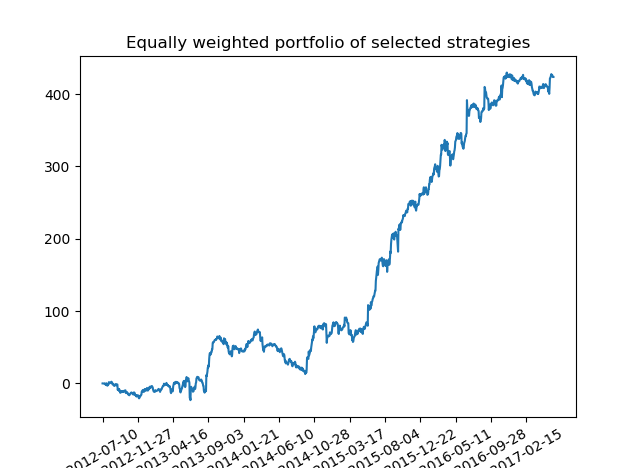
\includegraphics[width=0.6\textwidth]{Portfolio_Theory/Portfolio_Front_Figure_1.png}
	\captionof{figure}{Equally weighted portfolio of 50 strategies in the 75th percentile in terms of performance}
	\label{Equal_Weight_frontier}
\end{center}


It's sharpe is about 1.37, nothing special but at least it acts as a decent benchmark. Now let's try to build an efficient frontier from the calculations made before. We obtain the following efficient frontier in the $\sigma^2-\mu$ plan:

\begin{center}
	\centering
	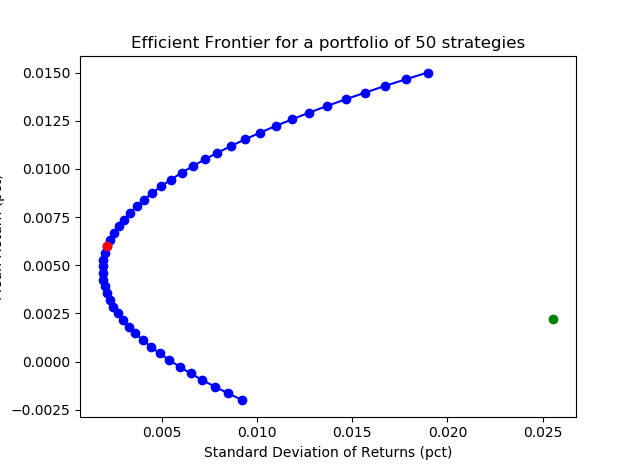
\includegraphics[width=0.6\textwidth]{Portfolio_Theory/Portfolio_Front_Figure_2.png}
	\captionof{figure}{Resulting portfolio frontier}
	\label{Frontier_frontier}
\end{center}

First of all we can spot the traditional parabolic shape of the portfolio frontier. The upper part of the portfolio frontier is referred to as the \textit{Portfolio Frontier}. We also highlighted two portfolios: the maximum sharpe ratio portfolio (red marker) and the equally weighted portfolio (green marker). We can clearly see how the equally weighted portfolio is non-optimal, with the same level of return we can substantially reduce our risk by finding a relative efficient allocation. The red spot is an interesing point, this portfolio is the one that achieves the maximum sharpe ratio, or in other words it provides the best tradeoff between risk and return. This portfolio can be obtained by analytical derivations, but in this case we just looked into the set of portfolios that we generated. In our project we will try to achieve this portfolio out-of-sample.\\
One important remark should be made before we move on: we will not be able to achieve the same level of optimality as we will not have the luxury of forecasting returns and variances.


\subsection{Why aren't Markowitz portfolios optimal?}

The title of this section sounds misleading, we just proved that optimal portfolios lie on the efficient frontier, why aren't they optimal then? Well the non-optimality is an issue that arises when we put the context of portfolio optimization in the real world. Some issues arise when portfolio managers try to optimize the weights relying solely on MPT's formulas. The underlying idea is really interesting, and this theory is still widely accepted as the cornerstone of portfolio optimization.\\
Let's see why such portfolios are not optimal in the real financial world, we will follow the outline provided in \cite{Critica_Markowitz}:

\begin{itemize}
	\item Markets change, in-sample and out-of sample are different
	\item Initially they had an issue of computational complexity that could not be solved, but modern computers can handle the level of computations required easily.
	\item Estimating the covariance matrix in absence of clean data, or a lot of data (especially if we have few samples and many assets) is a challenge and will be carried on with measurement errors. Nonetheless, Optimal portfolios are computed inverting the covariance matrix, this operation will amplify the degree of imprecision of the algorithm.
	\item As a result of the previous point, weights are highly unstable as time passes and this is a big issue for real-world large scale portfolios because of the difficulty of continuously rebalancing a big portfolio, but moreover because of the presence of relevant transaction costs. Transaction costs are a real-world friction that can really destry the good performance of an allocation method, even if the optimization has a good outcome, if the portfolio has to be continuously changed, trading fees will eat up most of the generated alpha.
\end{itemize}

This section has been put to add a critical overview of our objective, of course if these models where perfect we wouldn't bother putting an effort to develop something "more optimal". These statements ultimately justify our search for out-of-sample optimal portfolios.


\subsection{The risk-free asset}

At this point, In traditional books, the discussion on portfolios extends including risk-free assets. A risk-free asset is an asset that provides returns without any risk. That means that even in the worst case scenario this asset will pay back the invested capital and the accrued return or interest. As a result, the expected return on such an asset is lower than that of any stock or risky asset. A totally risk-averse investor will invest only in risk-free assets. Such an asset is usually considered to be a safe sovereign bond (core Europe bonds or US bonds) or bank accounts. There is still a little risk in them but the probability of defualt of such bonds is so little that they are usually considered as non risk-bearing. \\
In our analysis we will, ignore the existence of risk free assets since in our case the only risk-free alternative to investing in algorithmic trading strategies is to leave the cash uninvested at a zero interest-rate. In such a case, if we are risk-averse we would just not invest any money in the market.


\subsection{Performance Metrics}

Here comes a crucial part, we want to describe how we will assess the performance of our portfolio. We will aim at maximizing the out-of-sample Sharpe-Ratio and Sortino-Ratio. Let's analyze this statement piece by piece. The Sharpe-ratio is a well-known risk-adjusted performance measures that considers the average return of a portfolio divided by its standard deviation (ignoring risk-free assets in our case).\\
On the other hand, the Sortino-ratio is a performance measure that evaluates how much return does a portfolio give on it's standard deviation on certain days. Given $r_i$ the return on the i-th day, a precise formula is:

$$
Sortino = \displaystyle \frac{\sum\limits_{i=1}^N r_i}{\sum\limits_{j=1}^N (r_j - \mu)^2} \qquad j \in \mathcal{J}
$$ 

Where $\mathcal{J}$ is defined as the set of negative returns.\\
This means that we try to maximize returns without making their standard deviation grow too much. In particular maximizing a signal-to-noise ratio means maximizing the straightness of the PnL line. This is more than just maximizing the PnL because we want to have portfolios that are controllable in bad days and also scalable. The straightest the PnL line, the more we can increase the overall level of risk by just scaling the portfolio up in terms of traded sizes (within the limits given by the market). The idea of considering the standard deviation only in negative days is related to this fact, we want to control the standard deviation when things go in the wrong direction, avoiding our portfolio to incur in large drawdowns.




\section{Part 1: Strategy Selection}
%\addcontentsline{toc}{section}{Part 1: Strategy Selection}

\subsection{Problem Statement}
%\addcontentsline{toc}{subsection}{Problem Statement}

We give here an additional re-statement of the problem we try to tackle here. On each monday we have to allocate risk on each of the given strategies by choosing which ones to put into production for the following week. In an ideal world we would switch on all the strategies that will perform well during the following week and vice-versa with the bad ones. Unfortunately this is quite an impossible task, and we just seek a "statistical edge" that allows us to profit from appropriate selection of strategies on the long run.\\
For this first part we focus only on activating or de-activating the algorithms, we don't care about the risk weight to give to strategies (the output will be a $\{1,0\}$ signal).

\subsection{Building the Features}
%\addcontentsline{toc}{subsection}{Building the Features}

To be able to predict the performance of trading strategies we first need to build meaningful features that come out of a manipulation of the raw data. We start from simple performance metrics to advanced features computed on rolling windows. Here you can find a list with detailed information.

\begin{itemize} 
	\item \textit{Hit Ratio:} This feature computes the percentage of days with positive PnL over a certain rolling window. The higher the Hit Ratio, we expect that the higher the probability of positive returns in the future.\\ 
	
	\item \textit{Sharpe Ratio:}. This world-known measure comes as an evolution of the previous and is supposed to give some more information about the shape of the pnl line of a strategy. Intuition suggests that a strategy with high sharpe over long periods might continue providing gains in the foreseable future.\\
	
	\item \textit{Robust Sharpe Ratio} This feature is supposed to be a robust version of the sharpe ratio, computed trying to avoid the distorsive effects of outliers and measuremement errors. The formula is the following (given $\mathbf{r}$ of past returns):
	
		\begin{center} 
			$\displaystyle Robust\_Sharpe =  \frac{med(\mathbf{r})}{IQR(\mathbf{r})}$
		\end{center}
		
	Where $med$ stands for median and $IQR$ stands for interquantile range. Hopefully this feature should allow to ignore the non-normality of the distribution of returns and give a robust measure of performance.\\
	
	\item \textit{Exponetially Weighted Sharpe Ratio:}. This feature is an evolution of the simple sharpe ratio. It is computed as a roolling mean divided by a rolling standard deviation, calculated with exponential weighting. The rational between this choice is that an exponential sharpe should be able to capture faster changes in the evaluation of a performance of a strategy.\\
	
	  
	\item \textit{Performance Quantile:} This feature looks on a rolling window at the performance over a certain horizon. This past performance is averaged at a daily level and compared with the distribution of past returns. The are some interesting dynamics that this fature should capture. For example if a strategy that has been trading with very good performance over the last years suddenly stops being profitable, this feature will immediately advise to switch the strategy off. On the contrary, a strategy that has been performing poorly suddently records some good performance, resulting in a high position in the historical distribution and some risk being allocated in production.\\   

	\item \textit{Exponential Moving Average of PnL:} this feature is computed as the moving average over a certain period of the cumulative pnl line of a strategy weighted over history with exponential weighting. Given a time period $T$, a weight factor is computed as $k = \frac{2}{T+1}$ and the exponential moving average is computed as\\
	
	\begin{center} 
		$\displaystyle EMA[i] =  \left(pnl\_curve[i] - EMA[i-1]\right)k + EMA[i-1]$
	\end{center}
	
	Hopefully this feature should rapidly capture switching point in the performance of a strategy by looking at the difference betweek the pnl curve and its exponential moving average. An alternative could be to look at the crossing between moving averages, at the risk of switching late, but removing a good amount of noise.\\
	
	\item \textit{Tail Ratio:} This feature is computed as the ratio over a rolling window between the 95th and the absolute 5th percentile of the distribution of returns. The higher the tail ratio the more positively biased the distribution and the bigger the odds of getting positive weights by trading in the strategy. This feature has the really good characteristic of not being too sensitive to outliers allowing for a robust estimation of the strategy performance.\\
	
	\item \textit{Sortino Ratio:} Computed as the Sharpe ratio, but considering only the volatility of negative returns.\\ 
	
	\item \textit{Drawdown Mode:} This simple feature indicates whether a strategy is in drawdown or not. In other words it looks at the cumulative PnL of a given strategy and trades it when the current cumulative PnL is above the rolling max. More precisely, to give a bit more freedom in switching we allow the strategy to loose 2\% from the previous max before being switched off, to eliminate the effect of noise.\\
	 
\end{itemize}


\subsection{Relevant Features}
%\addcontentsline{toc}{subsection}{Relevant Features}	

Once the features have been built we have to decide which ones give the more predictive power to solve our problem. Moreover we need to assess which rolling window is ideal for any feature to be able to forecast at best. The approach chosen at this stage is to use a \textit{Random Forest} model to rank these features. The idea is to feed this model with all the possible features and let the algorithm select the best ones. To dig more in detail on how this process can be applied, a discussion of random forest trees is appropriate. A decision tree is a machine learning model that can predict quantitative and $\{0,1\}$ outputs given a set of features. The model takes binary decisions based on the input features partitioning the sample into different "leaves" and assigns output values minimizing the impurity that is a measure of homogenety of the data (See the appendix for greater detail on ow the algorithm works). Their use in feature selection is abundant thanks to their simple approach and their ability to model dependencies between features. If a tree, trained on some data, consistently splits based on the value of only one feature, it's a strong indication of importance of that feature. A Random forest uses the powerful concept of bootstrap on top of this model: it trains several trees, where any of these is trained only on a subset of the data sample and a subset of the features. The output is then the average split decision across all trees.\\
For our problem we even went further adapting this model to our specific dataset that has few data points (6 years of daily returns) for many different strategies. What we did is to use the powerful Python library \textit{Scikit Learn} to train a random forest on each of the 13000 strategies at hand (only in our train sample). Once the tree is trained we retrieve the feature importances and we sum them up across all the strategies. Each tree will be feeded with all the features computed above with different rolling windows (in our case 30, 60, 90, 120, 180, 210, 250, 300 days). Before going to the results, two important steps must be taken. The first is to compute an output feature on which the tree can actually train on. We decided to use a binary output ($0/1$) that tells whether the strategy has a positive (1) or negative (0) returns over the following 5 trading days. %We didn't limit the output to 5 trading days, even though it will be our final target, as the tree would have been subject to high noise, while the reliability of certain features should emerge on slightly longer terms.\\
The last part to take care of before training the model is to clean the data. We normalized the data, dropped extreme values and dropped strategies that had too few trading days, as these would haven't let the tree train properly. Moreover, to be consistent we restricted our study to the in-sample period.\\
Once the tree had been trained we recorded the most important features, these can be seen in Table \ref{table:feature}.

\begin{table}
	\centering
	\begin{tabular}{c|c}
		Feature & Importance \\\hline \hline
		Rolling Sharpe 350 & 0.04 \\ 
		Rolling Sharpe 250 & 0.0388 \\ 
		Rolling Sharpe 300 & 0.0387 \\ 
		Tail Ratio 60 & 0.0385 \\ 
		Tail Ratio 180 & 0.0385 \\ 
		Tail Ratio 90 & 0.0385 \\ 
		Rolling Sharpe 180 & 0.0385 \\ 
		Tail Ratio 120 & 0.0381 \\ 
		Rolling Sharpe 120 & 0.0379 \\ 
		Tail Ratio 350 & 0.0379 \\ 
		Tail Ratio 250 & 0.0378 \\ 
		Tail Ratio 300 & 0.0377 \\ 
		Rolling Sharpe 90 & 0.0373 \\ 
		Rolling Sharpe 60 & 0.0368 \\ 
		Exp Sharpe 350 & 0.0362 \\ 
		Exp Sharpe 60 & 0.0351 \\ 
		Exp Sharpe 300 & 0.0346 \\ 
		Exp Sharpe 250 & 0.0337 \\ 
		Exp Sharpe 90 & 0.0334 \\ 
		Exp Sharpe 180 & 0.0331 \\ 
		Exp Sharpe 120 & 0.033 \\ 
		Hit Ratio 350 & 0.0264 \\ 
		Hit Ratio 250 & 0.0264 \\ 
	\end{tabular}
	\caption{ Top 25 Features selected by the Random Forest Tree.}
	\label{table:feature}
\end{table}


We can see how the Sharpe-ratio dominates any other feature, establishing itself as the most powerful feature. Moreover we notice how the exponential moving average and robust Sharpe-ratio have very low predictive power. It is really interesting to observe how the relevance of features increases with the window, even if our aim is to predict over a very short period.\\
Once we agreed on the relevant features we started building a model to predict which strategies to put into production each week. We will not focus only on sharpe but we will still proceed in our work keeping in mind the hints given by this powerful tool.\\



\subsection{An Additional Test}

We want to check that the results coming from the Random Forest tree are actually meaningful. We specifically want to verify that the Sharpe ratio is not only just a better measure compared to a pool of features, but we want to ensure that Sharpe has significance at an absolute level. To this end, we will observe the problem from a slightly different angle. We want to verify whether the feature that is supposedly the best will actually have some predictive power for our portfolio.\\
To this end we will run a simple regression where we will try to predict the future one-week return of a strategy given one feature (the best one that is a rolling sharpe over a window of 350 trading days), in our case we will try to fit:

\begin{equation} \label{regression}
r_i = \beta SR\_350_i + \epsilon_i \qquad i=1\dots N
\end{equation}

Where N is the number of traded strategies. The regression is run on the whole in-sample period. We will evaluate the performance of the feature by looking at the $R^2$ score and the individual t-statistic.

\begin{figure}[htbp]
	\centering
	\includegraphics[width=0.6\textwidth]{Part_1/histograms.png}
	\caption{Empirical distribution of R-squared and t-statistics}
	\label{histograms}
\end{figure}

Remember that to accept the the alternative hypothesis of the feature being relevant at a 95\% level we need to have the t-statistic to be greater than 1.65.\\
We can clearly see how many strategies don't acknowledge the sharpe as a meaningful feature to predict future performance. In our case, there are also many strategies where this feature is definitely relevant. To add some significance to the chart, we report some numbers: 
roughly 10\% of the strategies have an r-squared that is greater than 10\%. On the other hand 37\% of all the strategies find the sharpe ratio as a relevant feature when the null hypothesis of non significance is tested against the alternative hypothesis of significance at a 95\% level.\\
This is a key piece of information, in fact we have a confirmation of the importance of this feature, but we also know that this doesn't apply to all the strategy, it cannot be elevated to the status of a "generic feature" that spots momentum on any strategy. 

\subsection{Switching Model}
%\addcontentsline{toc}{subsection}{Switching Model}

Here we dwelve into the challenge of finding an optimal subset of all the strategies to put in production for a given week. The model here should just tell us whether a strategy is good or bad for the coming week.\\
As opposed to a traditional machine learning model, we want something more simple, interpretable and faster. Following the results of our random forest tree classifier we decided to base our models on robust thresholds or ranking of strategies. The reasons for dropping cutting-edge machine learning methods in this context are multiple: first we don't have many samples per strategy to be able to train machine learning models. If we had more data, a Neural Network could for example learn the complex relationships between feature behaviour and future performance of the strategy, but since we have little amounts of data per strategy this could be hardly achievable. It is quite clear that in this context we are aiming at training individually each strategy, as trying to fit many different strategies in one model is definitely not optimal.\\
We have tested several different models and evaluated them based on the performance they provided. This performance is not only a function of raw PnL, but is at first risk-adjusted and secondarily it takes into account how volatile the allocation is. It is well established that some interesting theoretical models just don't work in the real world because of transaction-costs and implementation issues. We want to avoid falling into this problem, finding something that works really well in-sample but then requires to completely reshuffle the portfolio each week killing any kind of intrinsic alpha.
Each model will require to fit various parameters, therefore we will perform in-sample gridsearches looking for pseudo-optimal parameters trying to avoid overfitting. That means we will look at the results with common sense, if we will find very surprising numbers we will dwelve in the nature of these parameters, and eventually we might not validate the results we see.\\


\subsection{First Tests}
%\addcontentsline{toc}{subsection}{First Tests}

We run different tests (in our in-sample period) to see which meaningful combination of features could come up with a proper switching model. At first, we tried to base our models only on one feature and it turned out that using only one feature was not enough as the data is really diverse and many strategies have very poor performance. This fact forced us to somehow use a second feature to act as a filter that would wipe out of the full set of strategies a huge majority that had not been performing well in the past. We directed our endeavours towards finding this meaningful filter of strategies. What this filter has to do, is to look at the past performance of any single strategy and set a threshold below which even if the current performance is good this strategy would not be switched on. The reason for this is that many strategies have some very short period where they work well due to specific market conditions that don't last for long. We luckily have a huge wealth of strategies and we can afford being strict in selecting strategies giving more strength to our method. After some tests and discussions we decided that a good filter is given by a long-window rolling-sharpe ratio. This feature looks at the performance of a strategy and computes with a certain rolling window the Sharpe. Then we look at the resulting time series and we require the sharpe to be sufficiently good over a certain window in history. In other words, every Monday the historical x-days sharpe ratio for each strategy is computed and if we are able to find  a period of x-days when a strategy performed sufficiently well in terms of sharpe we believe this is a strategy that can be switched on and off in the future. Evidence will show that this lookback window should be quite long, proving that the strategy has been working for quite a long time in the past (See following parts). Once this filter is applied, the remaining features are switched according to information coming from another feature that we will explore in the following part.\\
Armed with this tool we started building many different models with all the features we had at hand. Results showed that the Random Forest tree was almost always right in estimating the predictive power of features. In fact, we noticed that portfolios based on features like Exponential Moving Averages and Hit Ratio (features with low predictive power) didn't perform as well as portfolios based on sharpe-ratio. We can see some results below:

\todo{METTI GRIDSEARCH CAGOSA}

Moreover, an interesting aspect to analyize is the set of strategies switched by these methods, it seems that they tend to select very similar strategies as the ones switched by the Sharpe-Ratio based portfolios, but with much worse market timing.\\

\subsection{Method 1: Pure Sharpe}
The first method we try is something really simple. We purely look at the Sharpe Ratio, we simply look for strategies that satisfied a certain requirement in the past and eventually select them based on the current Sharpe ratio over a certain window. More in detail, every week we scan the whole universe of strategies and we apply the aforementioned Sharpe-filter, pre-selecting only the ones that had a "good enough" performance over a certain window in the past. This period can be not in the near past. That means this is a strategy that somehow has proven to be an alpha generator in the past at least. After this pre-selection we put in production only the strategies that currently have a Sharpe-ratio over a certain window greater than a fixed threshold. For this method to work properly we need to fit four parameters (two thresholds and two windows for the Sharpe Ratio). Even though we might let the optimizer work on an infinite space, we set some boundaries to our search. For example, we will require the Sharpe filter to work over a longer period (at least 6 months). While the shorter Sharpe, will be based on a shorter window that will not exceed one trading year.\\
We run the in-sample grid search and nicely find a smooth surface. This is good news because it confirms that we are not chasing the noise but generating a real signal. 

\begin{center}
	\centering
	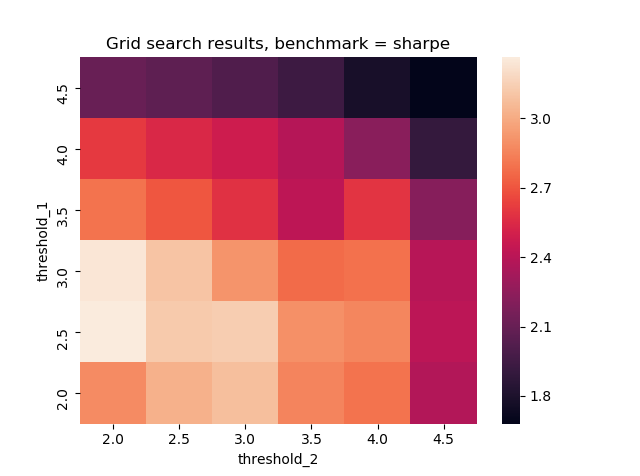
\includegraphics[width=0.6\textwidth]{GridSearches/Sharpe_Basic/Figure_1.png}
	\captionof{figure}{Grisearch results for the two thresholds}
	\label{Sharpe_Simple_1}
\end{center}

\begin{center}
	\centering
	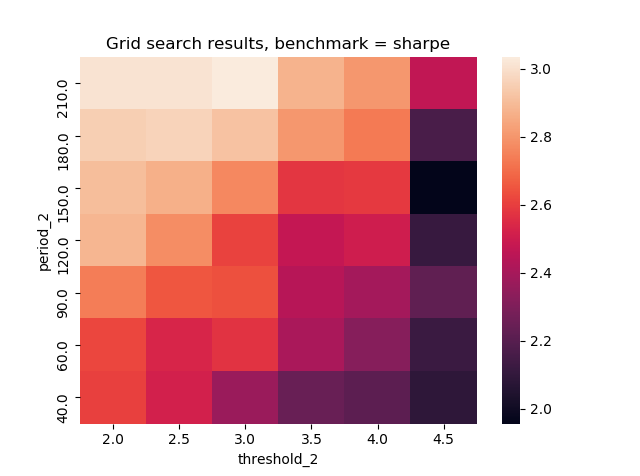
\includegraphics[width=0.6\textwidth]{GridSearches/Sharpe_Basic/Figure_2.png}
	\captionof{figure}{GridSearch for the threshold and period relative to the short Sharpe-Ratio}
	\label{Sharpe_Ranking_2}
\end{center}

\begin{center}
	\centering
	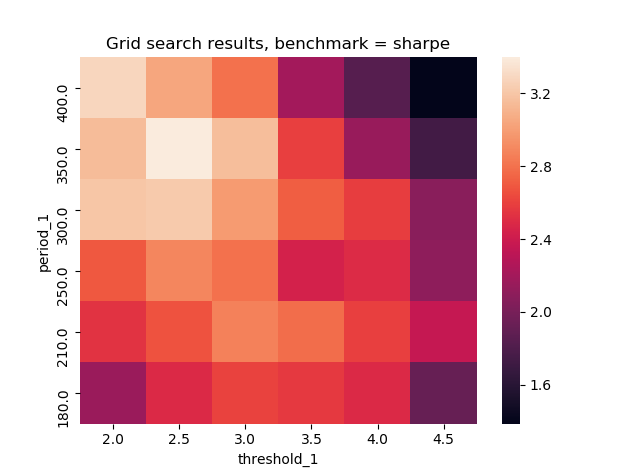
\includegraphics[width=0.6\textwidth]{GridSearches/Sharpe_Basic/Figure_5.png}
	\captionof{figure}{GridSearch for the threshold and period relative to the long Sharpe-Ratio}
	\label{Sharpe_Ranking_2}
\end{center}

The way these graphs should be interpreted is that for each point in the grid we see a value that is the average on all the possible values of the non displayed parameters. Otherwise we would have to draw somehow an n-dimensional cube, but for simplicity and visibility we prefer to plot everything on a 2D surface.\\

The results are definitely interesting. Since we don't care about finding exactly the perfect optimal combination of parameters we stick with what we believe makes sense in the optimal area that means longer Sharpe ratio over a period of 350 days and shorter Sharpe computed over a period of 210 days.



\subsection{Method 2: Ranking Based}
%\addcontentsline{toc}{subsection}{Method 2: Ranking Based}

We will propose an evolution of the basic case that reduces the search space and adds some robustness. The idea is that instead of swithcing strategies on and off based on the current short-term Sharpe-Ratio being above a certain threshold, we care about ranking the performance of strategies making the assumption that the best ones will still perform well. There are two reasons why this choice makes sense: first of all ranking removes the burden of optimizing some parameters reducing the risk of overfitting. Secondarily, ranking is a much more robust statistics than a simple threshold, we expect therefore that this method will perform better out of sample. We still have to apply a first filter as for the previous case (fixing the parameters as they have been chosen for method 1), then we will grid-search for an optimal window where strategies are ranked by Sharpe Ratio.\\
Notice that we also have to set a parameter that is the number of strategies that will be considered best ones after being ranked. The idea here is that this number is given by what the in-company execution system can withstand, that is about 50 strategies at the same time. More precisely we will select the top 50 strategies (out of 13000!) but only if their Sharpe-Ratio is still positive in the last period.

\begin{center}
	\centering
    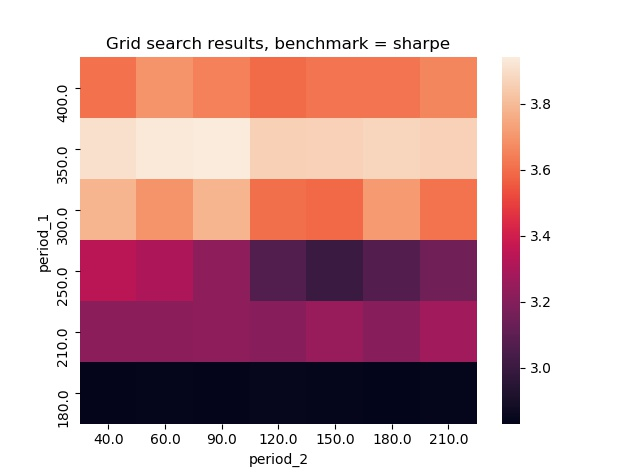
\includegraphics[width=0.6\textwidth]{GridSearches/Sharpe_Ranking/Figure_1.jpeg}
	\captionof{figure}{GridSearch for the two windows of the Sharpe Ratio}
	\label{Sharpe_Ranking_1}
\end{center}

\begin{center}
	\centering
	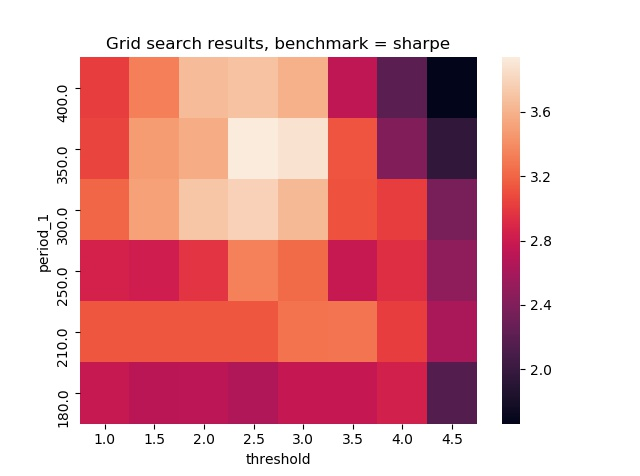
\includegraphics[width=0.6\textwidth]{GridSearches/Sharpe_Ranking/Figure_2.jpeg}
	\captionof{figure}{GridSearch for one window vs the threshold for the Sharpe Ratio}
	\label{Sharpe_Ranking_2}
\end{center}

\begin{center}
	\centering
	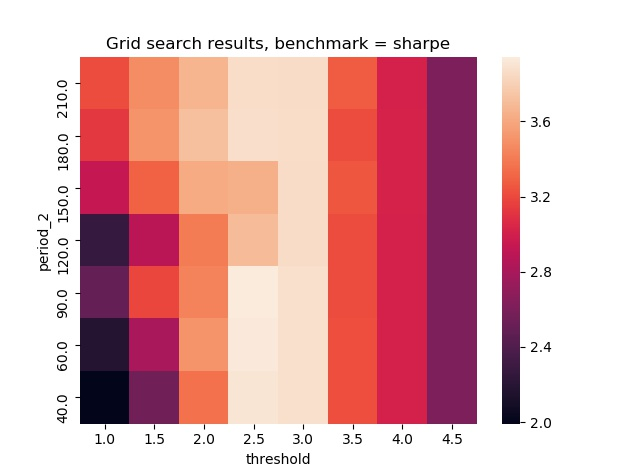
\includegraphics[width=0.6\textwidth]{GridSearches/Sharpe_Ranking/Figure_3.jpeg}
	\captionof{figure}{GridSearch for one window vs the threshold for the Sharpe Ratio}
	\label{Sharpe_Ranking_3}
\end{center}

As we can see the performance is on average much better, but also the results are more reliable. The in-sample gridsearch suggests that the optimal value for the filtering Sharpe is about 350 trading days, while for the threshold the ideal value seems to be in the 2.5/3 area. The length of the window for the Sharpe ratio used to rank doesn't seem to be extremely relevant but still it seems  to suggest that optimal values might be in the 90s.\\
Using these results we test the method in sample and obtain a nice equity line:

\begin{center}
	\centering
	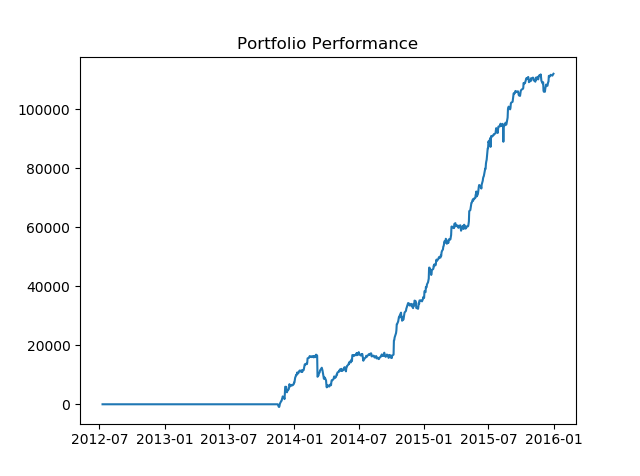
\includegraphics[width=0.6\textwidth]{GridSearches/Sharpe_Ranking/In_Sample_performance.png}
	\captionof{figure}{In-Sample performance for the Sharpe-ranking method}
	\label{Sharpe_Ranking_in_sample}
\end{center}

We can see that the statistics are quite good with an in-sample Sharpe-Ratio up to 3.69.

\begin{table}
	\centering
	\begin{tabular}{c|c}
		\textbf{Statistic} & \textbf{Value} \\\hline
		Sharpe Ratio & 3.696 \\ 
		Sortino Ratio & 4.2479 \\ 
		Omega Ratio & 2.13 \\ 
		Skewness & -0.6776 \\ 
		Kurtosis & 15.9628 \\ 
		Maximum Drawdown (\% duration/duration) & 14.4 \\ 
		Longest Drawdown (days) & 80.0 \\ 
		Winning Days & 63.3574 \\ 
	\end{tabular}
	\caption{\label{tab:widgets} Statistics for the in-sample performance of the Sharpe-Ranking method.}
\end{table}




\subsection{Method 3: Drawdown Based}

In this case we aim at finding something even more robust. Even though the Random Forest tree suggested that drawdown information is not as relevant as other features when it comes to predict the future performance of strategies, we decided to give a try to this feature as it is really robust and requires almost no parameter.\\
In detail, the model we try to create here will initially filter as we have seen in the previous two models, but then the remaining strategies will be put in production only if they are somehow showing a steadily growing equity line. In more mathematical terms, what we did is to compute the PnL line for each strategy and each week we see how much time the strategy has spent in drawdown in a certain window in the past. Then we take this number and divide it by the total length of the window. The underlying idea is that if a strategy has spent a lot of time in drawdown it might be that the underlying mean-reversion between traded assets is not working well, or simply it is exposed to significant PnL drops that is something the we really need to avoid. Anyway, the combination between Sharpe-ratio filter and drawdown information might give some additional alpha information to our portfolio construction so we decided to give it a shot. This idea of using drawdown information to forecast the performance of a strategy is not completely new, in fact some articles \cite{challet} invite to use drawdown information as a robust alternative to the Sharpe Ratio. The results for the in-sample gridsearches are as follows: 

\begin{center}
	\centering
	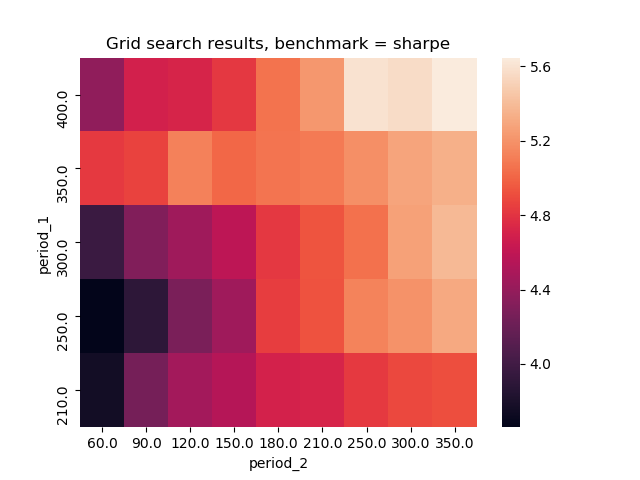
\includegraphics[width=0.6\textwidth]{GridSearches/Average_Drawdown/Figure_1.png}
	\captionof{figure}{GridSearch for the window of Sharpe Ratio and drawdown measure}
	\label{Average_Drawdown_1}
\end{center}

\begin{center}
	\centering
	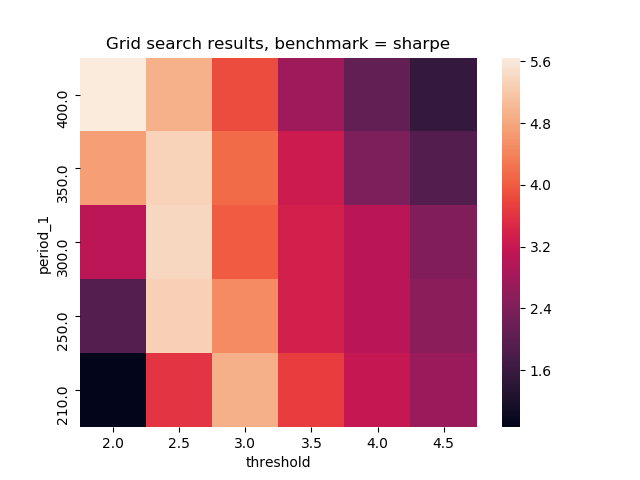
\includegraphics[width=0.6\textwidth]{GridSearches/Average_Drawdown/Figure_2.png}
	\captionof{figure}{GridSearch for the parameters relative to the Sharpe Ratio}
	\label{Average_Drawdown_2}
\end{center}

\begin{center}
	\centering
	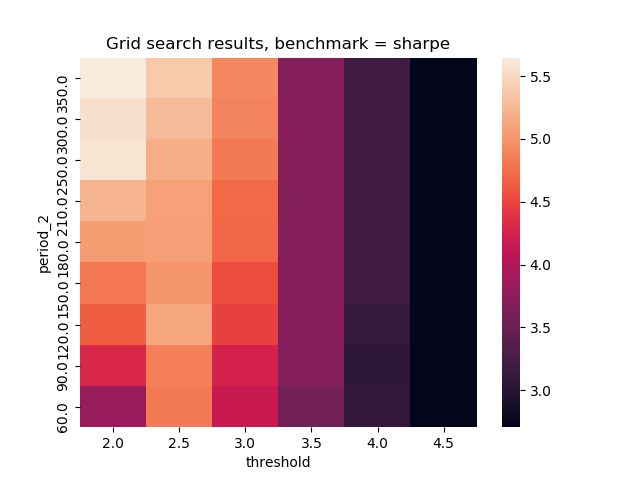
\includegraphics[width=0.6\textwidth]{GridSearches/Average_Drawdown/Figure_3.png}
	\captionof{figure}{GridSearch for drawdown window and sharpe threshold}
	\label{Average_Drawdown_3}
\end{center}

The optimal parameters are close to the ones we have seen for the second method, so we stick with them a part for the ranking period that is a bit longer in this case. Here you can see the resulting equity line:

\begin{center}
	\centering
	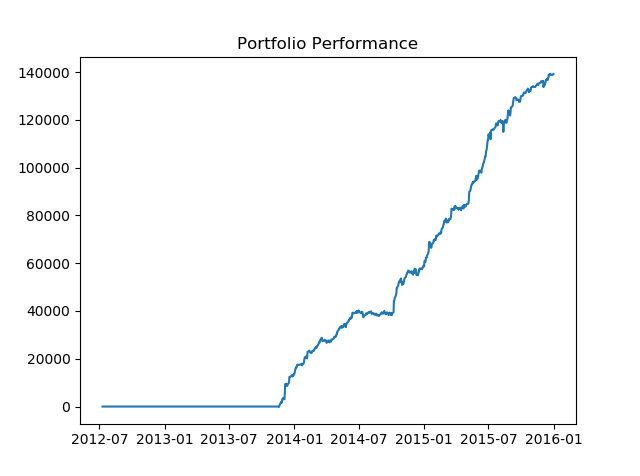
\includegraphics[width=0.6\textwidth]{GridSearches/Average_Drawdown/Average_Drawdown_In_Sample_Performance.png}
	\captionof{figure}{In-Sample performance for the Average-Drawdown method.}
	\label{Average_Drawdown_in_sample}
\end{center}

The statistics are the following:

\begin{table}
	\centering
	\begin{tabular}{c|c}
		\textbf{Statistic} & \textbf{Value} \\\hline
		Sharpe Ratio & 5.1853 \\ 
		Sortino Ratio & 7.7506 \\ 
		Omega Ratio & 2.81 \\ 
		Skewness & 0.8184 \\ 
		Kurtosis & 7.5674 \\ 
		Maximum Drawdown (\% duration/duration) & 12.7 \\ 
		Longest Drawdown (days) & 70.0 \\ 
		Winning Days & 64.557 \\ 
	\end{tabular}
	\caption{\label{tab:widgets} Statistics for the in-sample performance of the Average-Drawdown method.}
\end{table}

The performance is definitely better than that of a plain sharpe-based method, it seems like if we use more precise and/or cleaner information. Therefore our Sharpe ratio increases by 2 units in terms of performance that is really good. 

\subsection{Method 4: Regression}

Here we detail our most complex experiment. This time we aimed to (almost) cancel any kind of dependence from parameters. The idea is that we will let a regression chose whether to switch a strategy on or off. The potential advantages of such methods are multiple: in fact reducing the dependence from parameters we basically cancel the possibility of overfitting, while letting a model work on the processed information allows to extract more information out of the PnL curve. We will not try any complex Machine Learning method as we don't want something very obscure and hard to interpret, but moreover we need something extremely fast. The idea is that every Monday we will fit a linear model to the data available up to that day, then we will make a prediction looking at the data we have at that current moment in time. If the prediction is good we will put the strategy in production, otherwise we will leave it switched off.\\
The linear model that we will fit is the following:

\begin{equation} \label{OLS}
r_i = \alpha + \beta_1 Sharpe_{long,i} + \beta_2 Sharpe_{mid,i} + \beta_3 Sharpe_{short,i}  + \epsilon_i 
\end{equation}

Where $r_i$ stands for the daily return of a trading strategy and the various Sharpe ratios stand for a rolling sharpe computed on the data up to that day. With this model we aim to capture information from long and short term together. Of course there are some details to be fixed before proceeding. For example the OLS framework assumes that our data is normally distributed, unfortunately as we noticed in section 2 our data is not Gaussian. Each day we will standardize our data with mean and variance available up to that day, in this way our regression will be more meaningful.\\
There is an additional layer of filtering that we want to use, and it is relative to the fact that not all strategies can be suitably switchable with this model, what we will do then is to require for each regression that we run to have at least one of the $\beta s$ of the regressions to be statistically significant at a 95\% level(i.e. with a t-stat of at least 1.65).\\
This model is definitely more robust, the only parameter we have is the threshold on the prediction of the regression used to define a strategy as "good", but it will be calibrated in a way that we reach a certain number of strategies in production. The other parameters are the windows of the Sharpe ratios, but these are quite simple to choose once we have seen the results of the Random Forest, it makes sense to take as windows for the three Sharpe ratios 350, 180 and 60 respectively.\\
One last  consideration to be made is relative to a weak point of this method, since we are regressing many strategies, our model will take a long time to be backtested. For each backtest (in-sample) we roughly have to run $13000 \cdot 395 = 5135000$ regressions.\\
But let's move to explore the results of this model. 

\begin{table}
	\centering
	\begin{tabular}{c|c}
		\textbf{Statistic} & \textbf{Value} \\\hline
		Sharpe Ratio & 2.235 \\ 
		Sortino Ratio & 2.5471 \\ 
		Omega Ratio & 1.53 \\ 
		Skewness & -0.7782 \\ 
		Kurtosis & 11.20 \\ 
		Maximum Drawdown (\% duration/duration) & 10.6 \\ 
		Longest Drawdown (days) & 88.0 \\ 
		Winning Days & 61.47 \\ 
	\end{tabular}
	\caption{\label{tab:widgets} Statistics for the in-sample performance of the Regression based method.}
\end{table}

We can see that unfortunately the robustness given by this model is not matched by a good performance as well. Even though the method might be good we decided to drop it due to the bad performance it provides.  

\begin{center}
	\centering
	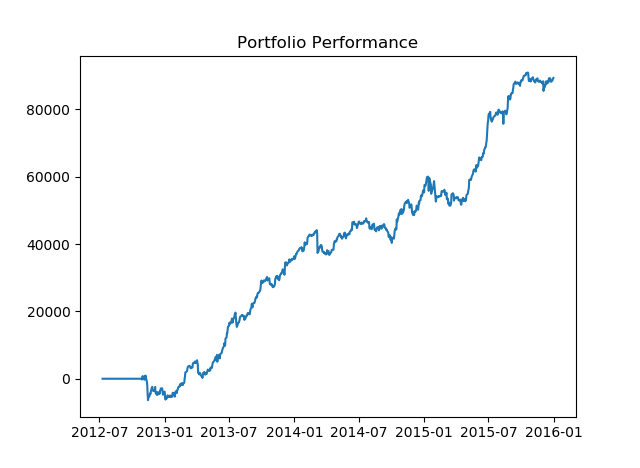
\includegraphics[width=0.6\textwidth]{GridSearches/Regression_Based/in_sample_performance.png}
	\captionof{figure}{In-sample performance of the Regression based method}
	\label{Average_Drawdown_3}
\end{center}


\begin{center}
	\centering
	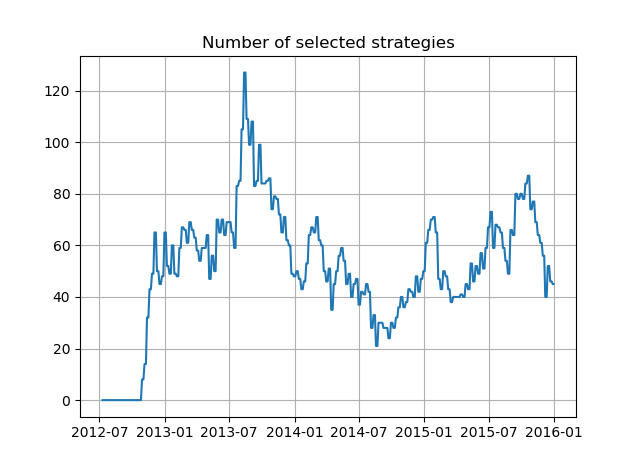
\includegraphics[width=0.6\textwidth]{GridSearches/Regression_Based/num_strats_in_sample.png}
	\captionof{figure}{Number of strategies selected each week by the Regression based method.}
	\label{Average_Drawdown_in_sample}
\end{center}

As we can see, here we select more strategies than before, but the performance is still subject to many drops that really make us not favour this model over the other ones.

\section{Part 2: Risk Allocation}

Once we have a robust and trustable switching method, we can move our scope towards risk minimization, or in more precise terms, sharpe ratio maximization. We will build on top of the selected portfolio two different weights systems that will be benchmarked against a simple equally weighted portfolio and a Markowitz-like minimum variance portfolio (see appendix for building details). As it was for the switching problem, our aim is still to find the best out-of-sample portfolio for the following week (setting the new weights on monday) given information up to the previous friday. \\

\subsection{Model 1 - A Genetic Learner}

The first method we try to implement is a Genetic-Learning portfolio allocator. The method is based on the idea of making the algorithm evolve to find an optimal allocation through extensive genetic mutation. \todo{DESCRITTO DA QUALCUNO, CITA ATRICOLI} The approach is rather brute-force as it tries to test as many portfolios as possible until the optimal one is found. This method allows to look for an optimal portfolio in a very different approach from what is usually done in the literature. A more human-like analogy is the following: the algorithm acts as a boss letting many portfolio managers allocate risk according to their views. As time passes the boss will evaluate the portfolio managers based on specific performance measures (that are not only raw pnl) and kicks out the worst performing. At each stage he tries to replace the worst portfolio managers with completely new ones and with a set of managers that trade similarly to the best ones. Let's dig into the underlying methodology: on each Monday we face the challenge of assigning weights (between 0 and 1) to the set of tradable strategies. The algorithm is initialized  with a set of random portfolios $\mathbf{w} = (\mathbf{w_1} \dots \mathbf{w_N})$, where each $\mathbf{w_1}$ represents a feasible allocation of risk (we will generate uniformly distributed random weights where 1 represents the maximum risk that can be allocated to a strategy and zero means that no risk is allocated to the strategy). The algorithm lets these portfolios trade over a certain window in the past and evaluates their performance. Once all of them have traded, the algorithm ranks them assigning a score given by a so-called \textit{Fitness Function}, which takes many metrics into account to evaluate a portfolio. Then the algorithm kicks out the worst performing, and substitutes them with a new generation (details on this part will be explained later).\\ 
The procedure is repeated until an optimum is reached, or in other terms this optimizer is not able to find better portfolios. At this point the final portfolio will be an average of the best found portfolios.\\
The name Genetic comes from the idea that natural selection and evolution are applied to the set of portfolios. If a portfolio is just bad it will not survive the selection step, while if a portfolio is good it will be challenged with a muted version of itself that might represent an evolutional step. This kind of approach has pros and cons, let's first evaluate the positive aspects:
\begin{itemize}
	\item The optimization is carried in a way that is able to be conducted in a multidimentional space, in different local minima in parallel avoiding the risk of missing a global minimum. The mutation happens in a way that optimization is more refined in well performing areas, while it is also randomized to cover the whole space
	\item The algorithm is conceived in such a way that it serves really well our needs and requirements. Evaluating portfolios with the so called Fitness Function it allows to penalize portfolios that perform well but that give rise to the typical issues of portfolio optimization like instability of weights, poor diversification or meaningless negative weights. The optimization is already done without having to worry about any type of complex mathematical formulation to impose constraints.
	\item The approach requires very little parameters: the length of the lookback window and the weights to give to any performance measure used to assess portfolio performance.
	\item The algorithm might fully embrace the non-linearity of the problem and autonomously find relationships between strategies that other methods might not find. 
\end{itemize}  

On the other hand this method has some drawbacks:

\begin{itemize}
	\item This brute-force algorithm requires an enormous computing power to span the whole space and rank all the portfolio. Needless to say, we will notice later that the more computing time is given to the algoithm the more the randomness in it is limited and the performance improves. We will dig later in this aspect. 
	\item As outlined above, there is some randomness, as most of the portfolios that are tested are just randomly generated, so there is little chance to find a precise optimum, but rather something that is quite close to it.
	\item The algorithm looks backward and makes the assumption that the best performing combination in the past will still be the best for the next week, so in a certain sense it goes around the issue of forecasting by making this simple assumption. Moreover this lookback window is a parameter that might require optimization.
	\item Even though there are few parameters to be set and the algorithm is not so sensitive to these values, the optimization requires a long time and some intuition to find meaningful numbers.
\end{itemize}


\subsubsection{Implementation}

Let's now address the issue of defining the fitness function. We will indicate this function with the symbol $f_f$, it is a simple $\mathbb{R}^N \rightarrow \mathbb{R}$ that given a portfolio vector $\mathbf{w}$ returns a real number as a score. This function is the core of the whole algorithm, because it can evaluate a portfolio based on its performance but also based on how the portfolio fits our requirements. This core function will look for a particular optimum that is charachterized by a portfolio vector that scores well according to different metrics. For example it might penalize a portfolio that assigns a lot of weight to few strategies, or a portfolio that changes too much compared to what was traded the previous week. Defining this function in the proper way takes more intuition than calculation, and requires to pay attention to a couple of details. Of course, the more complex the fitness function the more our taste can be satisfied, but also the more computational time is required.\\

\todo{Qui metti tipo di randomizzazione/replacement}\\
\todo{Metti dettagli per definire l'ottimo}\\

\subsubsection{Fitness Function}

We will evaluate the performance of the portfolio based on a mix of sharpe ratio and sortino ratio (achieved over a certain lookback period), somehow taking into account the diversification benefit of a portfolio allocation. We will also take into account how much a portfolio will be different from the previous one with a norm-1 penalty.
So our fitness function will look like:\\

$$
f_f = \alpha_1*sharpe(\mathbf{w}) + \alpha_2*sortino(\mathbf{w}) - \alpha_3*||\mathbf{w} - \mathbf{w_{old}}||
$$

Where $\alpha_1$, $\alpha_2$, and $\alpha_3$ are weights on which no optimization will be carried to limit the computaional burden. $\alpha_1$ and $\alpha_2$ will be the same, while $\alpha_3$ will be such that the influence on the optimal portfolio is relevant but still not that big to prevent the portfolio form evolving towards ones with better performance. In other wordsd, if an optimal portfolio is really different from the one traded the previous week, it must mean that the performance of the former must be really good to make us switch towards it incurring in relevant transaction costs.\\ 
We need to assign proper values for those three parameters in a way that it makes sense. We will give more relative weight to performance measures such as sharpe and sortino ratios and a bit less to the stability of the portfolio. To do this we take into account the order of magnitude of our scores. The sharpe ratio will be in absolute value normally in the range between 0 and 1.5 (we will not annualize the ratios as we care only about comparing performances, this way we will save some computations). The sortino ratio will be in the range between 0 and 3 in the most realistic cases.\\
For wat concerns the order of magnitude of the 1-norm we need to dig into some mathematics. We will generate the random weights for each portfolio manager as uniform values in the range $[0,1]$. The value of the norm-1 will be the sum of the absolute value of the difference of N uniform random variables. We will compute in the end the expected value of this norm-1. Let's set $\mathbf{X}, \mathbf{Y} \stackrel{i.i.d.}{\sim} \mathcal{U}(0,1)$.\\
\begin{equation} \label{first_step}
\mathbb{P}\left(\left\lVert\mathbf{X} - \mathbf{Y}\right\rVert < k\right) = \mathbb{P}\left(\mathbf{X} - k < \mathbf{Y} < \mathbf{X} + k\right)
\end{equation}  
We can easily visualize this simple problem on the $\mathbf{X}-\mathbf{Y}$ plane.\\

\begin{center}
	\centering
	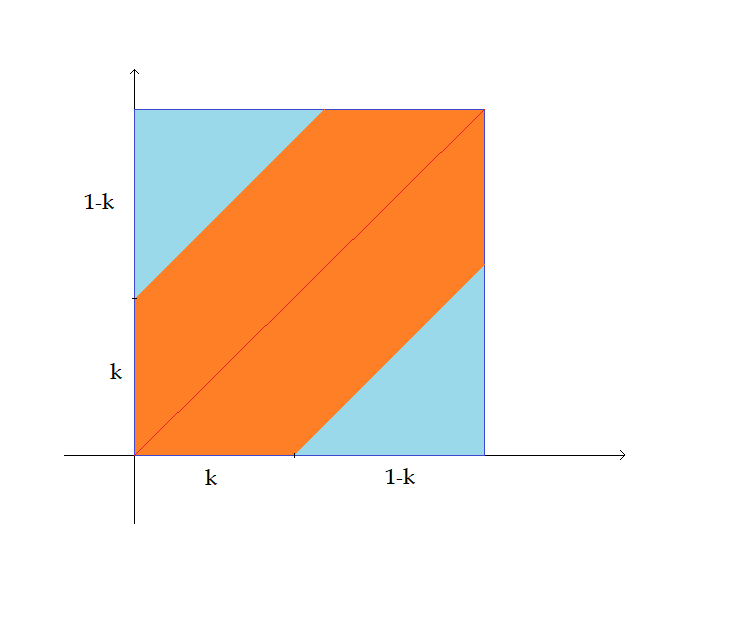
\includegraphics[width=0.6\textwidth]{Genetic_Algo/Prob_Square.png}
	\captionof{figure}{X-Y plane representation of the problem}
	\label{X_Y_plane}
\end{center}

The red area represents out probability. It is quite straightforward to notice that the area is equal to $1 - (1-k)^2 = 2k - k^2$. We can now extract the pdf of this particular random variable:

\begin{equation} \label{pdf}
f_{\left \lVert \mathbf{X} - \mathbf{Y}\right\rVert}(k) = \frac{dF_{\left \lVert \mathbf{X} - \mathbf{Y}\right\rVert}}{dx} = 2 - 2k \mathbf{1}_{[0,1]}(k)
\end{equation}

Now we can compute the expected value with the normal laws of probability:

\begin{equation} \label{expected_value}
\mathbb{E}\left[\left \lVert \mathbf{X} - \mathbf{Y}\right\rVert\right]  = \int_0^1 kf_{\left \lVert \mathbf{X} - \mathbf{Y}\right\rVert}(k)dk = k^2 - \frac{2}{3}k^3 \Big| _0^1 = \frac{1}{3}
\end{equation}

So the expected value of the norm difference for any portfolio will be $\frac{N}{3}$, where N is the number of assets in the portfolio (each week these are roughly 50-60). This means that this third element will be much greater in magnitude than the performance measures. We will need to set a value for $\alpha_3$ about 20 times smaller than $\alpha_1$ and $\alpha_2$. Since the scores will be relative to each other we don't care about the scale of the values, but only about the relative sizes. We therefore decide to set $\alpha_1 = \alpha_2 = 0.5$ and subsequently $\alpha_3 = 0.025$. 




\subsubsection{Converging towards a global optima}


Now let's address the issue of how to reach a global optima. The algorithm has its specific way of finding an optimal allocation that is derived from evolutionary theory. The idea is that each of the original portfolios are tested, but only the best ones will survive to the next period. These ones will evolve in modifications of the original portfolios and will face the challenge of surviving against a new random generation of portfolios. More specifically the procedure is the following:

\begin{itemize}
	\item First N portfolios are randomly generated. The bigger N the more extensive the search and higher the probability of actually finding an optimal point. This of course comes at a larger expense of optimization time.
	\item Each portfolio is evaluated through the fitness function, so that portfolios can be ranked based on this score.
	\item then a \textbf{selection} step is enforced. Only the best k\% of the portfolios survive, these portfolios will make it to the next optimization round. k is usually in the 20-50\% range, and we will stick to a 30\% value. Moreover, these portfolios are selected to breed a new generation.
	\item The new generation is created through the process of \textbf{mutation}, that means that each portfolio is generated as a little variation of one of the best pre-existing portfolios. An alternative here is \textbf{crossover} that mimics the dynamics of reproduction in the human world. In this case two portfolios would be "mixed" to give birth to a new portfolio. Here we have different alternatives of how to create the crossover, one can just average to portfolios, or select some genes randomly from the two portfolios and so on. For our case we believe mutation works better as we need a faster and simpler method to generate portfolios. Moreover averaging or mixing portfolios would bring us towards almost equally weighted portfolios that we want to avoid since we really want to force our algorithm to search for more extreme and exhotic combinations. 
	\item The remaining part of the set is generated again in a random fashion and the loop starts again.
\end{itemize}

This procedure will hopefully bring to an optimal portfolio. We need to decide how to define an optimal point, or in other words establish when should the optimization terminate. There are many different ways to establish a termination condition, common ones are to stop once a certain performance criteria is reached (i.e a minimum Sharpe Ratio), or to stop the optimization after a fixed amount of time/iterations. Our procedure will be a bit more complex, we will let the evolutionary process continue until a minimum number of iterations will have been done and the improvement in the top portfolios is not that relevant so that it is worth carrying the optimization on. We can see in the following chart a snapshot of an optimization procedure, as we increase the number of iterations the best elements improve their performance until they reach a level where increasing the number of iterations doesn't bring any value to the portfolio.\\

\todo{Chart dell'evoluzione di f\_record}

We now aim to show how this optimization process works in an intuitive and visual way. We consider the optimization process for one date and show the evolution of the various generations of portfolios. We use a nice heatmap where every colour indicates a different "species". At each iteration the species are sorted by score and it is easy to see how as the optimization process goes on some species become dominant and mark the evolution of most of the portfolios.

\todo{Metti foto heatmap optimization}

\subsection{Model 2 - An enhanced risk-parity}

Here we propose an alternative model, here we look for something more controllable, interpretable and less computationally heavy. The idea is to oppose the genetic learner with something particularly different.\\
If we look at the drawbacks of Genetic Portfolios described in section 4.1, we will be able to overcome them here. In fact, the computational power required is much lower, the solution is exact in the sense that there is no randomness here but moreover there are very few parameters in the algorithm, and the dependency on these parameters is not that relevant.\\
Let's dig a bit in how this portfolio is going to be built. As an alternative to the genetic portfolio, we will start from the same point, that is a given allocation of strategies for a given week. We will try to achieve a minimum variance approach, of course for all the reasons outlined above we will not try to use directly a Markowitz approach (even though this will be considered as a benchmark). Given an allocation we will try to minimize the risk by looking for similar strategies and penalizing their weight in production to avoid having a portfolio that has an excessive exposure to a certain sector/region/asset-class. This should ideally give a well-diversified portfolio. We will at last look at the sharpe ratio to tilt the weight towards better performing strategies.\\
More in detail our approach will be:

\begin{itemize}
	\item Get the strategies in production, look at their PnL history and reduce them with a PCA to $n_dim$ dimensions.
	\item Use this reduced data to cluster the strategies based on their PnL. In this way we avoid the use of correlation that is tricky and numerical error-prone. The algorithm that will be used to perform this clustering is detailed in the next section. The good thing about this algorithm is that we don't need to set a parameter for the number of clusters to create.
	\item Apply equal weights to each cluster, that means that if there is a big cluster of many similar strategies, these will be put with a low weight to keep the portfolio diverisified.
	\item Tilt the weights based on the sharpe ratio.
\end{itemize}

\subsubsection{Clustering the strategies with affinity propagation}

\subsubsection{Allocating risk}



\section*{Results}

\section*{Appendix}
\addcontentsline{toc}{section}{Appendix}


\subsection*{Shapiro-Wilks normality test}
\addcontentsline{toc}{subsection}{Shapiro-Wilks normality test}

As suggested by the name, the Shapiro-Wilks test checks if a sample is drawn from a normal distribution. More precisely, given a sample it tests $H_0$ (normality) versus the alternative hypothesis of non-normality. This test is ideal for our case as it doesn't require too much data to come to a conclusion. The test is non parametric and starts with sorting the data. Once the data is sorted, the test statistic can be computed:

$$
\displaystyle W = \frac{\left(\sum\limits_{i=1}^N a_{i}x_{(i)}\right)^2}{\sum\limits_{i=1}^N(x_i-\bar{x})^2}
$$

Each element has its specific meaning:
\begin{itemize}
	\item $\bar{x}$ is the sample mean of the data.
	\item $x_{(i)}$ is the $i$-th order statistic. 
	\item $a_i$ are tabulated coefficients coming out of the distribution of order statistics of a normal standard distribution.
\end{itemize}

The larger the statistic the more "normal" the data. This comes from the idea that the test wants to measure the similatity of the ordered statistics to those of a standard normal distribution. The W statistic somehow measures the closedness of these two entities.

\subsection*{Minimum Variance Portfolio}
\addcontentsline{toc}{subsection}{Minimum Variance Portfolio}

Here we build the foundations of the Minimum Variance portfolio used as a benchmark to measure the relative performance of our weight assignment methods.\\
Firstly, we set the problem in rigorous terms: given a set of N tradable instruments (in our case trading strategies) we want to find the optimal trading vector $\mathbf{w} = (\mathbf{w_1} \dots \mathbf{w_N})$ that represents the composition of our portfolio. This composition will optimally be the one that minimizes the in-sample variance of the portfolio. The latter is measured as:

$$
\sigma^2_\pi = \frac{1}{2} \mathbf{w}^T\mathbf{\Sigma} \mathbf{w}
$$

This optimization problem is usually solved under the constraint that the sum of the weights should be equal to one. We will solve the problem and then impose that the weights are also positive (it wouldn't make sense to trade strtegies with negative weights).\\
The lagrangean to solve to minimize the variance is the following:

$$
\mathbf{L} = \frac{1}{2} \mathbf{w}^T\mathbf{\Sigma} \mathbf{w} - \lambda\left(\mathbf{1}^T\mathbf{w} - 1\right)
$$

Where $\mathbf{1}$ is a vector made up of ones.\\
We compute the first order conditions:

$$
\frac{\partial \mathbf{L}}{\partial \mathbf{w}} = \mathbf{\Sigma} \mathbf{w} - \lambda\mathbf{1} = 0 \qquad  \frac{\partial \mathbf{L}}{\partial \lambda} = \mathbf{1}^T\mathbf{w} - 1 = 0
$$

From the first F.O.C. we immediately find:

$$
\mathbf{w} = \lambda \mathbf{\Sigma}^{-1} \mathbf{1}
$$

We plug this result into the other F.O.C.:

$$
\lambda \mathbf{1}^T \mathbf{\Sigma}^{-1} \mathbf{1} - 1 = 0 \Longrightarrow \lambda = \frac{1}{\mathbf{1}^T \mathbf{\Sigma}^{-1} \mathbf{1}}
$$

Therefore getting a nice analytical closed-form solution for our minimum variance portfolio:

$$
\mathbf{w} = \frac{\mathbf{\Sigma}^{-1} \mathbf{1}}{\mathbf{1}^T \mathbf{\Sigma}^{-1} \mathbf{1}}
$$

The beauty of this formula comes with some drawbacks:
\begin{itemize}
	\item $\mathbf{\Sigma}$ is often not precisely estimated due to the huge number of strategies and the little amount of samples to use to measure standard deviations and correlations. Moreover this matrix is not to invert leading to numerical errors. To partially address these issues we use a \textit{LedoitWolf} covariance matrix whose construction is explained in the next chapter.
	\item This approach completely ignores transaction costs, leading to a fastly changing and unstable portfolio composition
	\item The model works making a basic assumption: in-sample correlations and variances will hold out-of-sample with very simila values. Unfortunately this is rarely the case in the real world, making this portfolio sub-optimal in terms of variance.
\end{itemize}

\subsection*{Ledoit Wolf Covariance Matrix}
\addcontentsline{toc}{subsection}{Ledoit Wolf Covariance Matrix}

\subsection*{Random Forest Tree}
\addcontentsline{toc}{subsection}{Random Forest Tree}

As outlined before, the decision trees are an all-purpose machine learning algorithm able to be trained on extremely non-linear phenomena. The beauty of these algorithm lies in the simplicity of the underlying learning process, the data is split in "sectors" in a way that the highest "purity" is achieved. The Random forest algorithm adds robustness to this process. Let's first explore in detail the training process for a simple decision tree.\\

\begin{itemize}
	\item  Given an m-dimensional set of data with an output feature (we are in the case of supervised learning) examine all the possible splits on one feature.
	\item Evaluate each split based on the purity of the splitted areas. This is done trough the \textit{Gini} impurity measure: $I_G = \sum\limits_{i=1}^N p_i(1-p_1)$, where $N$ is the number of labels/classes in the data.\\
	Ths measure indicates how often a randomly chosen element from the set would be incorrectly labeled if it was randomly labeled according to the distribution of labels in the subset. This comes clear with the fact that the tree assigns probability to labels.
	\item The purest split gives rise to a new node.
	\item From this split others are generated until the highest purity or the maximum number of splits is achieved.\\
\end{itemize}

As it might emerge from this brief explanation, decision trees tend to overfit the data, as they learn very complex non linear-features. This behaviour is described in the context of the bias-variance trade-off where decision trees stand more in favor of variance rather than bias. Random forest try to overcome this issue by averaging many trees.\\
Once we understood how a general decision tree is trained we can explore in depth the training of a random forest algorithm:

\begin{itemize}
	\item Generate M different trees.
	\item Each tree is trained (as a normal decision tree) on a random subset of the features. This number is usually believed to be a fraction $\sqrt{n}/n$ where $n$ is the number of features.
	\item The results from all the trees are averaged, that means that for each point the final label will be given by the average of all labels given by the different M trees. 
\end{itemize}

This robust procedure is useful to train powerful regressors or classifiers, but might be used as well to measure the forecasting ability of the input features. If a feature has real predictive power, it will be used in many bootstrapped samples to produce splits in the data, therefore being used many times. Computing the number of times each feature is used to produce a split will give a ranking of feature importances.\\

\newpage
%\section*{Appendix}
\subsection*{Figures and Tables}

\begin{figure}[htbp]
	\centering
	\includegraphics[width=0.6\textwidth]{Figures/moving_average.eps}
	\caption{Rolling average of the returns for 4 industries and Rf}
	\label{rolling_average}
\end{figure}








\clearpage

\begin {table}[htbp]
\begin{center}
\input{Figures/industry_summary.tex}
\end{center}
\caption {Descriptive statistics for simple returns} \label{industry_summary} 
\end {table}



\newpage
%\clearpage

\bibliographystyle{unsrt} 
\bibliography{Biblio}



\end{document}
